
\chapter{Business Applications Domains}
\label{appendix:design:domain:services_contexts}

The developed \gls{PoC}s are:

\begin{itemize}
      \item Smart Irrigation;
      \item Fleet Management;
      \item Notification Management.
\end{itemize}

Each of this services' models will be briefly addressed in the following sections. The shared model presented above defined the structure and semantic of incoming data. Each service then uses the shared model how they envision, in their specific practical and pragmatic fashion.

\section{Fleet Management}
\label{subsubsec:design:domain:bounded_contexts:fleet}

The \textbf{Fleet Management} model simply refers to the past and current location of assets.

The diagram in Figure~\ref{fig:design:domain:bounded_contexts:fleet:diagram} displays the noteworthy concepts related to this service.

\begin{figure}[H]
   \centering
   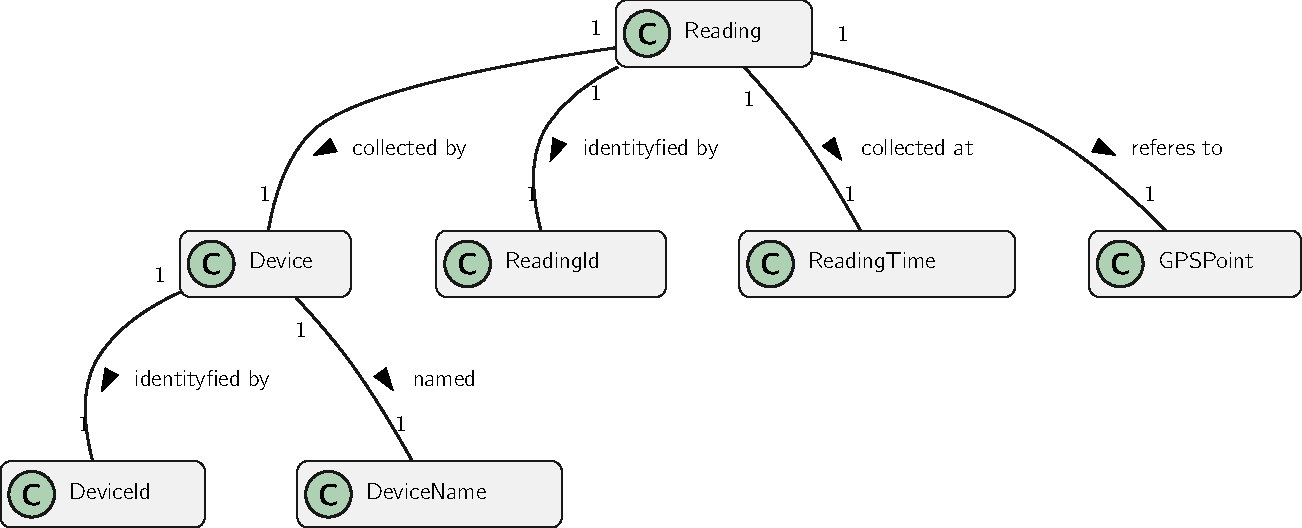
\includegraphics[page=1,width=\columnwidth]{assets/diagrams/design/domain/fleet-management-model.pdf}
  \caption[Fleet Management Model]{Fleet Management Model}
  \label{fig:design:domain:bounded_contexts:fleet:diagram}
\end{figure}

This was the first Business Application built as a \gls{PoC}, it was intended to be straightforward. The model references \gls{GPS} readings and what device collected them.

\section{Notification Management}
\label{subsubsec:design:domain:bounded_contexts:notification}

The \textbf{Notification Management} model refer to notifications and how/what types an addressee wants to receive. There are two main concepts in this service, a notification and an addressee.

The diagram in Figure~\ref{fig:design:domain:bounded_contexts:notification:diagram} displays the noteworthy concepts related to this service.

\begin{figure}[H]
   \centering
  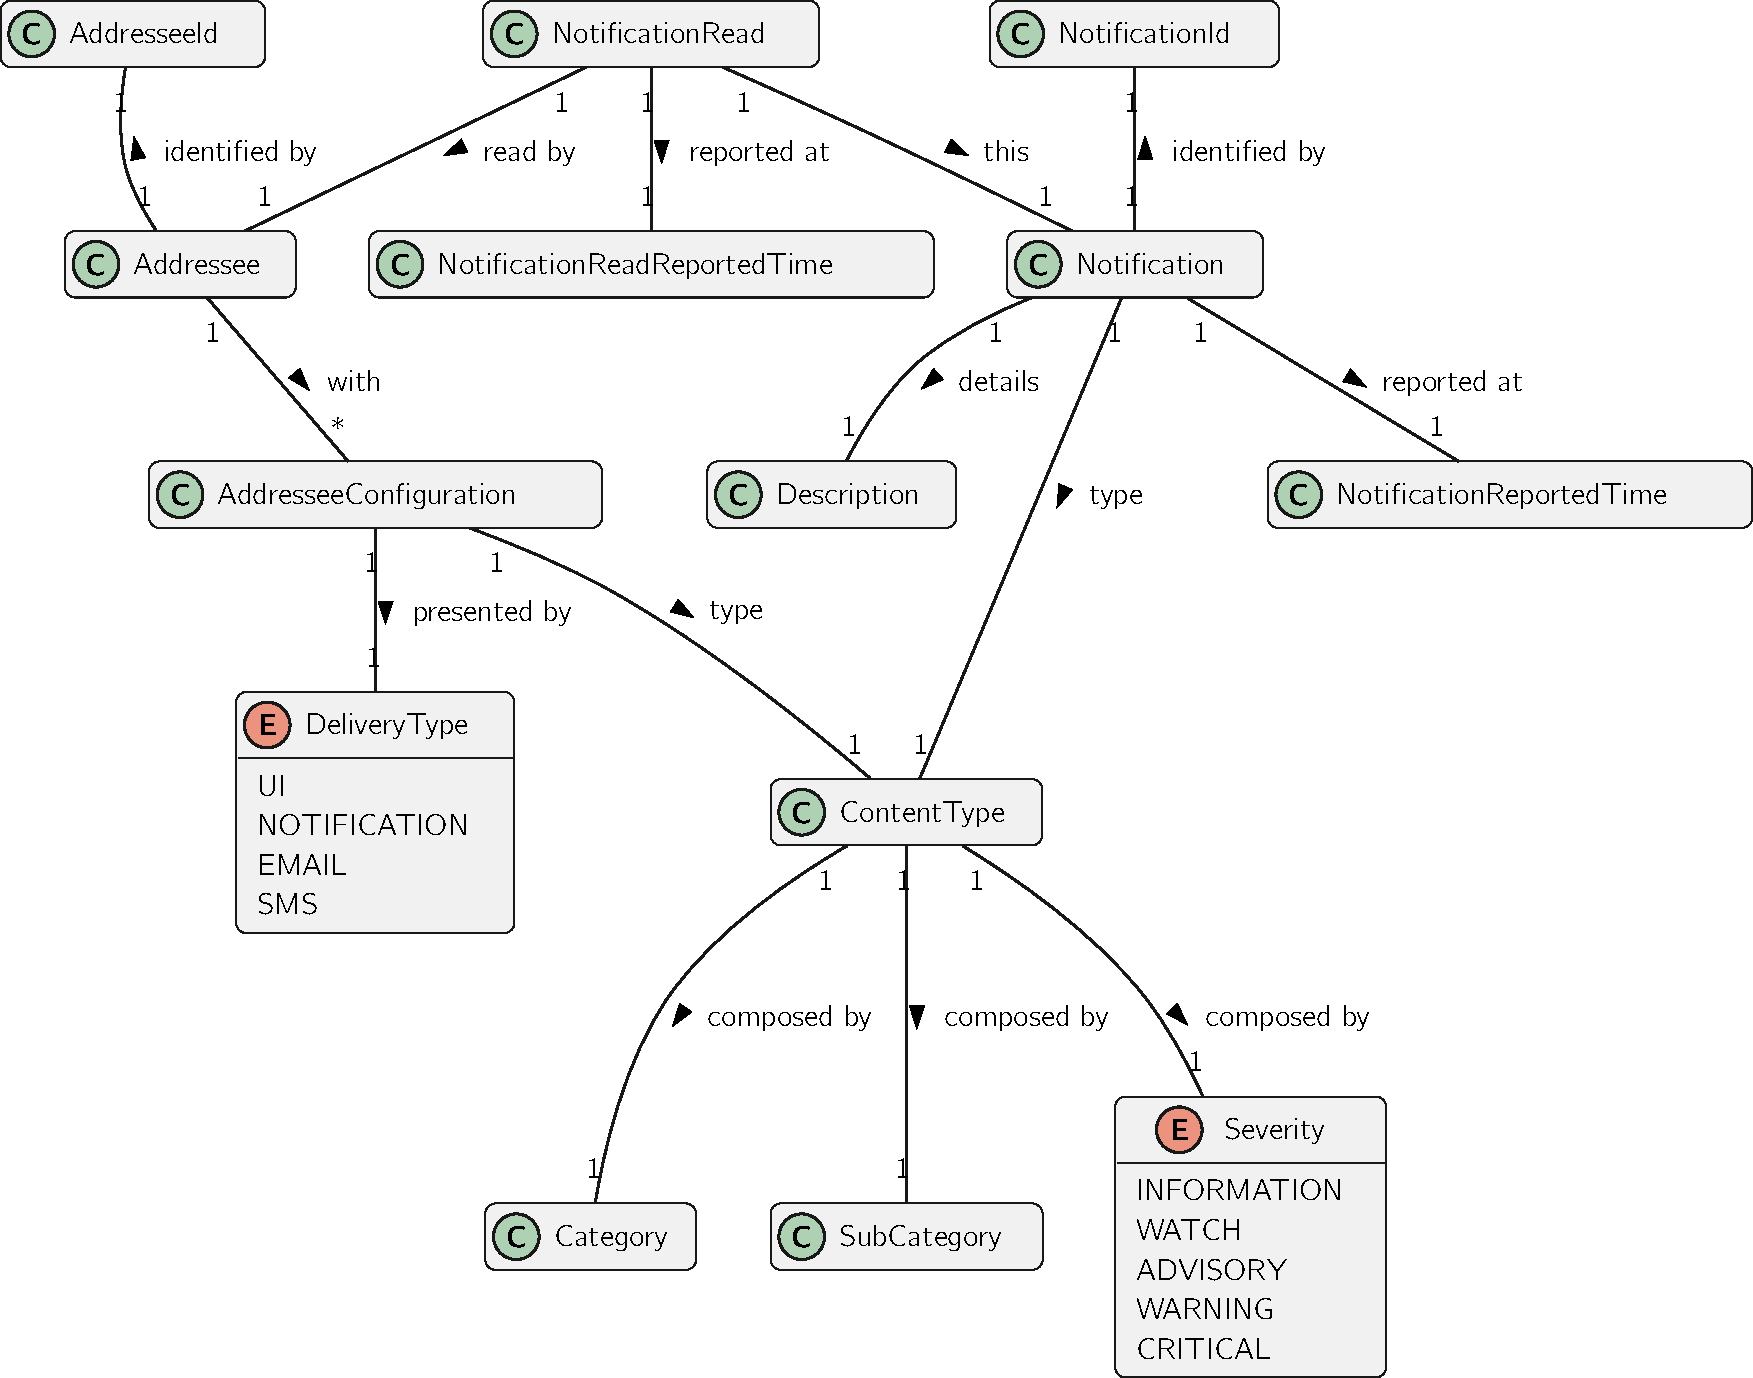
\includegraphics[page=1,width=\columnwidth]{assets/diagrams/design/domain/notification-management-model.pdf}
  \caption[Notification Management Model]{Notification Management Model}
  \label{fig:design:domain:bounded_contexts:notification:diagram}
\end{figure}

As a brief description:

\begin{itemize}
   \item A \textbf{Notification} is a sanitized \textbf{Alert} that was captured with the intent to be presented or delivered to addressees, its identified by an \textbf{NotificationId};
   \item An \textbf{Addressee} is someone that receives notifications based on his configurations and is identified by an \textbf{AddresseeId};
   \item An \textbf{AddresseeConfiguration} defines for each type of notification - \textbf{ContentType} - what will be the delivery method - \textbf{DeliveryType};
   \item A \textbf{DeliveryType} can be of four types: (i) present in SPA - \textbf{UI}, (ii) publish notification in SPA - \textbf{NOTIFICATION}, (iii) send an email - \textbf{EMAIL}, (iv) send an SMS - \textbf{SMS};
   \item A \textbf{ContentType} is derived from the \textbf{Alert} Routing Keys mentioned in the Table~\ref{tab:design:domain:shared_model:routing} and defines the type of each \textbf{Notification};
   \item To enforce accountability in the system, the notion of who read a specific notification and when was added - \textbf{NotificationRead}.
\end{itemize}

\section{Smart Irrigation}
\label{subsubsec:design:domain:bounded_contexts:irrigation}

The \textbf{Smart Irrigation} model refers to irrigation zones, sensors that read environmental conditions in this zones, valves and the associated readings. This concepts are divided in three diagrams presented below.

The diagram in Figure~\ref{fig:design:domain:bounded_contexts:irrigation:diagram:garden} displays the noteworthy concepts related to irrigation zones.

An irrigation zone is an area intended to function as an isolated environment that may or may not have valves or sensors.

\begin{figure}[H]
   \centering
   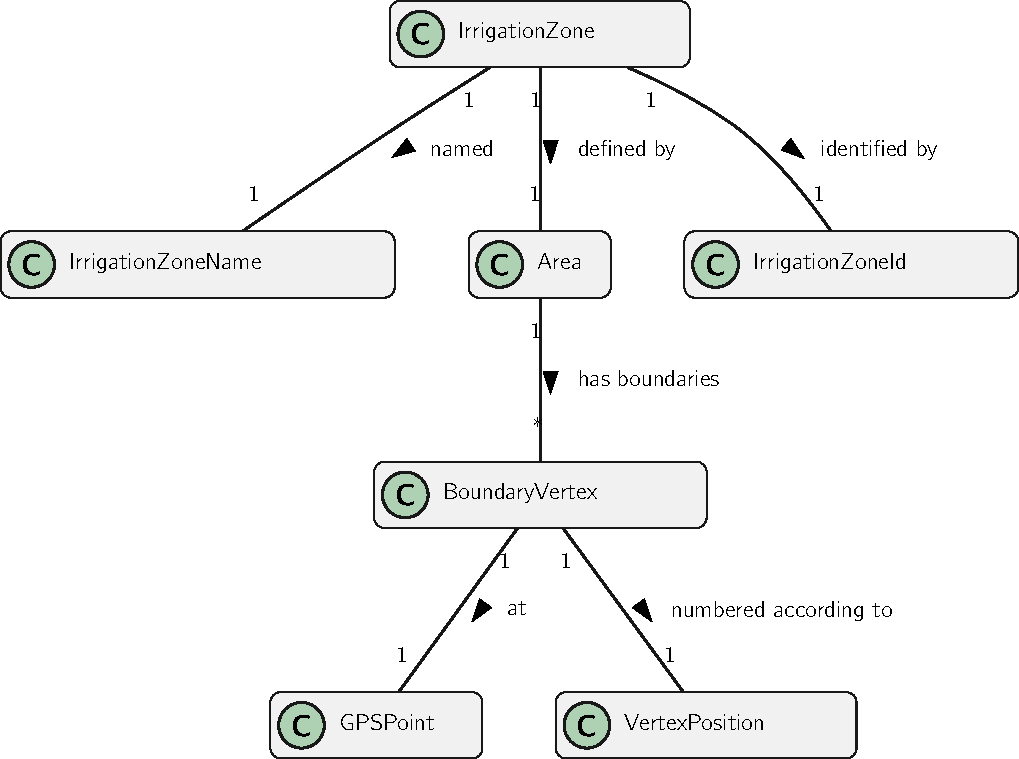
\includegraphics[page=1,width=0.7\columnwidth]{assets/diagrams/design/domain/smart-irrigation-model-2.pdf}
  \caption[Smart Irrigation Model - Irrigation Zone]{Smart Irrigation Model - Irrigation Zone}
  \label{fig:design:domain:bounded_contexts:irrigation:diagram:garden}
\end{figure}

A sensor or valve belongs to an irrigation zone if it is inside the zone's \textbf{Area}.

As presented in the following diagram, Figure~\ref{fig:design:domain:bounded_contexts:irrigation:diagram:device}, a sensor/valve can be represents by a \textbf{Device}.

\begin{figure}[H]
   \centering
  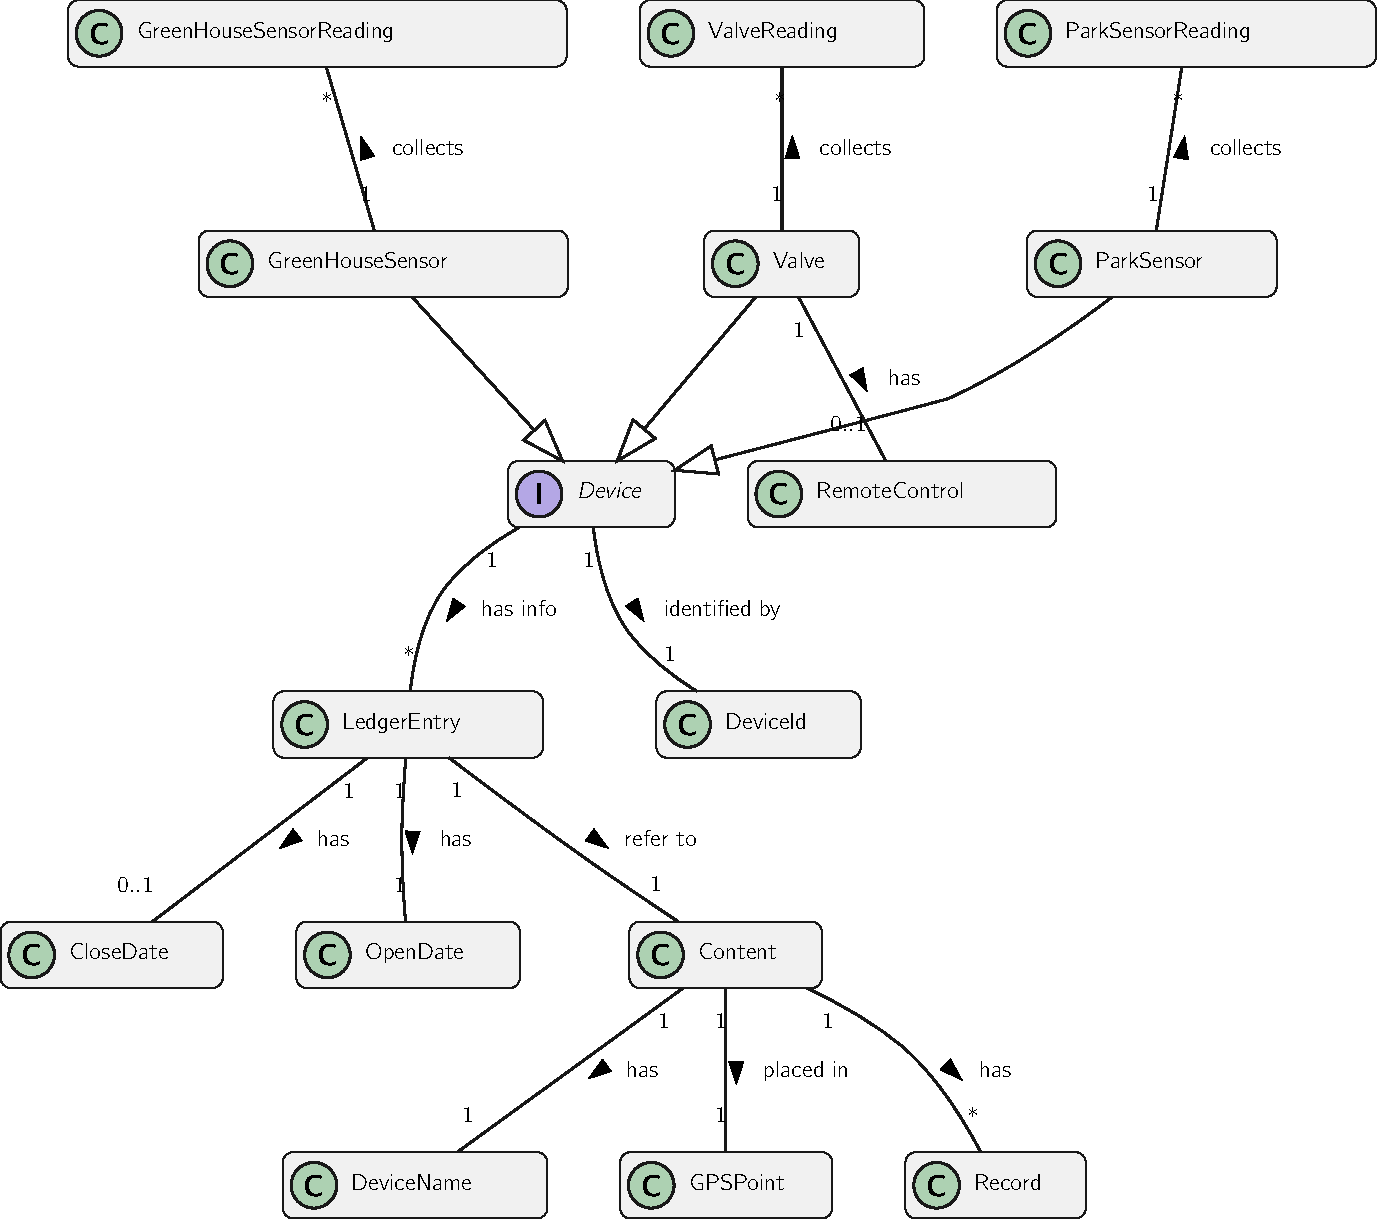
\includegraphics[page=1,width=\columnwidth]{assets/diagrams/design/domain/smart-irrigation-model-3.pdf}
  \caption[Smart Irrigation Model - Device]{Smart Irrigation Model - Device}
  \label{fig:design:domain:bounded_contexts:irrigation:diagram:device}
\end{figure}

As a brief description:

\begin{itemize}
   \item The \textbf{RemoteControl} defines if a \textbf{Valve} can be controlled remotely. A valve can be controlled remotely only if two specific types of \textbf{Command}s (as defined in the \nameref{subsec:design:domain:shared_model}) are sent with the device's \textbf{Data Unit}: \textit{OpenValve} and \textit{CloseValve};
   \item A \textbf{Device} is identified by its \textbf{DeviceId};
   \item Each \textbf{Device} stores an history of all its changes such as name, location or metadata in \textbf{Content}, the same \textbf{LedgerEntry} is used as long as this values don't change;
   \item There are three types of \textbf{Device}: (i) Green House Sensor, (ii) Park Sensor, (iii) Valve. Each of this types collect different measures discussed in Figure\ref{fig:design:domain:bounded_contexts:irrigation:diagram:reading}.
\end{itemize}

As mentioned above each type of device collects different readings. The following diagram, Figure\ref{fig:design:domain:bounded_contexts:irrigation:diagram:reading}, details this readings.

\begin{figure}[H]
  \centering
  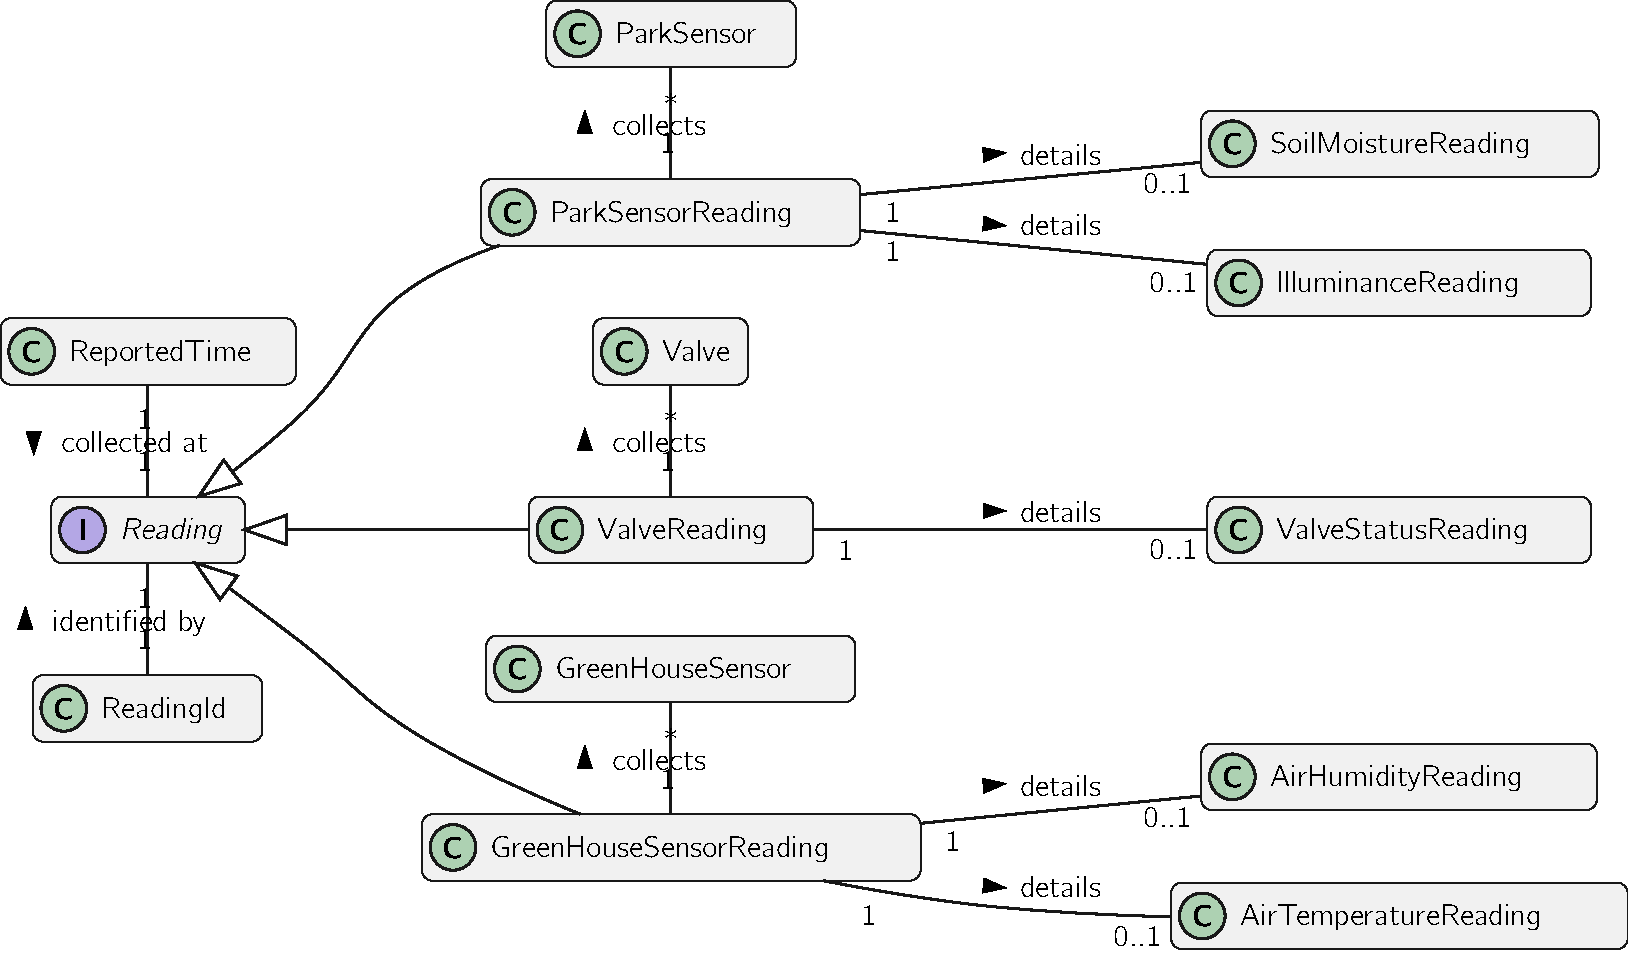
\includegraphics[page=1,width=\columnwidth]{assets/diagrams/design/domain/smart-irrigation-model-4.pdf}
  \caption[Smart Irrigation Model - Reading]{Smart Irrigation Model - Reading}
  \label{fig:design:domain:bounded_contexts:irrigation:diagram:reading}
\end{figure}

As a brief description:

\begin{itemize}
   \item A \textbf{Reading} is always identified by its \textbf{ReadingId} and is associated to the instant that it was captured by the \textbf{Device} - \textbf{ReportedTime};
   \item A \textbf{ParkSensorReading} measures soil moisture and illuminance;
   \item A \textbf{Valve} indicates if it is open or closed;
   \item A \textbf{GreenHouseSensor} measures air humidity and air temperature.
\end{itemize}

The concepts in this last diagram are different from the concepts in the other two diagram since readings data is suppose to be immutable and ample as opposed to devices and irrigation zones where information should be mutable but with a negligible size compared with readings.
